% FULL PAPER (IEEE two-column conference format). Sections follow the course template:
% Abstract, Introduction, Literature Review, Problem Statement, Methodology, Results and
% Discussion, Conclusion. Build: `uv run qdrift paper --build` (tectonic) or upload the whole
% paper/ folder to Overleaf. The interim report (first three sections only) is interim.tex.
%
% WRITING RULES (similarity check < 15%):
%  - Write every sentence yourself. Do not paste from papers, the reading log or AI tools.
%  - Quote rarely, one short sentence at most, in quotation marks, with \cite.
%  - Delete the guidance comments (%) before submission and run scripts/check_paper.py.
\documentclass[10pt,conference]{IEEEtran}
% Shared by main.tex (full paper) and interim.tex (Introduction, Literature Review and Problem
% Statement only). Numbers come from generated/numbers.tex through \val{key}; tables and figures
% come from generated/. Never type a result by hand.
\IEEEoverridecommandlockouts
\usepackage[T1]{fontenc}
\usepackage{cite}
\usepackage{amsmath,amssymb}
\usepackage{array}
\usepackage{graphicx}
\usepackage{booktabs}
\usepackage{xcolor}
\usepackage[hidelinks]{hyperref}
\graphicspath{{generated/figures/}}

% Generated by `uv run qdrift paper`; do not edit.
\providecommand{\qdset}[2]{\expandafter\def\csname qd@#1\endcsname{#2}}
\qdset{acc-EMU-breastcancer-M1}{0.963}
\qdset{acc-EMU-breastcancer-M2}{0.907}
\qdset{acc-EMU-breastcancer-M3}{0.883}
\qdset{acc-EMU-twocurves-M1}{0.917}
\qdset{acc-EMU-twocurves-M2}{0.760}
\qdset{acc-EMU-twocurves-M3}{0.797}
\qdset{acc-R0-breastcancer-M1}{0.887}
\qdset{acc-R0-breastcancer-M2}{0.893}
\qdset{acc-R0-breastcancer-M3}{0.837}
\qdset{acc-R0-twocurves-M1}{0.813}
\qdset{acc-R0-twocurves-M2}{0.707}
\qdset{acc-R0-twocurves-M3}{0.647}
\qdset{acc-R1-breastcancer-M1}{0.893}
\qdset{acc-R1-breastcancer-M2}{0.893}
\qdset{acc-R1-breastcancer-M3}{0.807}
\qdset{acc-R1-twocurves-M1}{0.800}
\qdset{acc-R1-twocurves-M2}{0.663}
\qdset{acc-R1-twocurves-M3}{0.670}
\qdset{acc-R216-breastcancer-M1}{0.887}
\qdset{acc-R216-breastcancer-M2}{0.897}
\qdset{acc-R216-breastcancer-M3}{0.830}
\qdset{acc-R216-twocurves-M1}{0.803}
\qdset{acc-R216-twocurves-M2}{0.727}
\qdset{acc-R216-twocurves-M3}{0.663}
\qdset{acc-R216s1-breastcancer-M1}{0.887}
\qdset{acc-R216s1-breastcancer-M2}{0.897}
\qdset{acc-R216s1-breastcancer-M3}{0.830}
\qdset{acc-R216s1-twocurves-M1}{0.803}
\qdset{acc-R216s1-twocurves-M2}{0.727}
\qdset{acc-R216s1-twocurves-M3}{0.663}
\qdset{acc-R232-breastcancer-M1}{0.887}
\qdset{acc-R232-breastcancer-M2}{0.893}
\qdset{acc-R232-breastcancer-M3}{0.813}
\qdset{acc-R232-twocurves-M1}{0.810}
\qdset{acc-R232-twocurves-M2}{0.713}
\qdset{acc-R232-twocurves-M3}{0.643}
\qdset{acc-R28-breastcancer-M1}{0.883}
\qdset{acc-R28-breastcancer-M2}{0.893}
\qdset{acc-R28-breastcancer-M3}{0.830}
\qdset{acc-R28-twocurves-M1}{0.800}
\qdset{acc-R28-twocurves-M2}{0.703}
\qdset{acc-R28-twocurves-M3}{0.663}
\qdset{acc-R3m-breastcancer-M1}{0.897}
\qdset{acc-R3m-breastcancer-M2}{0.897}
\qdset{acc-R3m-breastcancer-M3}{0.860}
\qdset{acc-R3m-twocurves-M1}{0.827}
\qdset{acc-R3m-twocurves-M2}{0.727}
\qdset{acc-R3m-twocurves-M3}{0.667}
\qdset{acc-R3r-breastcancer-M1}{0.907}
\qdset{acc-R3r-breastcancer-M2}{0.907}
\qdset{acc-R3r-breastcancer-M3}{0.843}
\qdset{acc-R3r-twocurves-M1}{0.810}
\qdset{acc-R3r-twocurves-M2}{0.673}
\qdset{acc-R3r-twocurves-M3}{0.663}
\qdset{acc-R4-breastcancer-M1}{0.890}
\qdset{acc-R4-breastcancer-M2}{0.897}
\qdset{acc-R4-breastcancer-M3}{0.827}
\qdset{acc-R4-twocurves-M1}{0.817}
\qdset{acc-R4-twocurves-M2}{0.750}
\qdset{acc-R4-twocurves-M3}{0.683}
\qdset{acc-SIM-breastcancer-M1}{0.967}
\qdset{acc-SIM-breastcancer-M2}{0.933}
\qdset{acc-SIM-breastcancer-M3}{0.913}
\qdset{acc-SIM-twocurves-M1}{0.927}
\qdset{acc-SIM-twocurves-M2}{0.873}
\qdset{acc-SIM-twocurves-M3}{0.847}
\qdset{aci-gamma}{0.03}
\qdset{alpha}{0.1}
\qdset{base-acc-breastcancer-logreg}{0.940}
\qdset{base-acc-breastcancer-mlp}{0.960}
\qdset{base-acc-breastcancer-rbfsvm}{0.940}
\qdset{base-acc-twocurves-logreg}{0.733}
\qdset{base-acc-twocurves-mlp}{0.973}
\qdset{base-acc-twocurves-rbfsvm}{0.987}
\qdset{bootstrap}{2,000}
\qdset{budget-cap}{1200}
\qdset{campaign-cap}{400}
\qdset{campaign-first}{2026-10-27}
\qdset{campaign-last}{2026-10-27}
\qdset{coverage-target}{90\%}
\qdset{devices}{\texttt{ibm\_fez} and \texttt{ibm\_kingston}}
\qdset{emulator-shots}{2000}
\qdset{fallback}{\texttt{ibm\_marrakesh}}
\qdset{gap-max-pp}{22.7}
\qdset{gap-mean-pp}{11.3}
\qdset{gap-min-pp}{4.0}
\qdset{h1-decision}{supported}
\qdset{h1-hi}{0.105}
\qdset{h1-lo}{0.044}
\qdset{h1-mean}{0.074}
\qdset{h3-decision}{not supported}
\qdset{h3-hi}{0.029}
\qdset{h3-lo}{-0.001}
\qdset{h3-mean}{0.013}
\qdset{h4-decision}{not supported}
\qdset{m1-features}{4}
\qdset{m1-layers}{3}
\qdset{m1-params}{28}
\qdset{m1-restarts}{3}
\qdset{m1-steps}{200}
\qdset{m2-features}{12}
\qdset{m2-layers}{1}
\qdset{m3-features}{10}
\qdset{m3-layers}{2}
\qdset{n-cal}{32}
\qdset{n-hw-samples}{182}
\qdset{n-qubits}{4}
\qdset{n-test}{150}
\qdset{n-train}{240}
\qdset{n-val}{100}
\qdset{noise-aware-shots}{2,000}
\qdset{patch-buffer}{1}
\qdset{patches}{14}
\qdset{per-execution-us}{265}
\qdset{pilot-cap}{90}
\qdset{qpu-campaign}{41}
\qdset{qpu-pilot}{22}
\qdset{qpu-used}{63}
\qdset{queue-max-h}{1.9}
\qdset{queue-median-h}{1.0}
\qdset{readout-shots}{2000}
\qdset{refit-lambda}{0.25}
\qdset{seed}{20261026}
\qdset{session-usage-mean}{20.5}
\qdset{sessions-done}{2}
\qdset{sessions-per-device}{5}
\qdset{sessions-planned}{10}
\qdset{shots}{500}
\qdset{sim-acc-breastcancer-M1}{0.967}
\qdset{sim-acc-breastcancer-M2}{0.933}
\qdset{sim-acc-breastcancer-M3}{0.913}
\qdset{sim-acc-twocurves-M1}{0.927}
\qdset{sim-acc-twocurves-M2}{0.873}
\qdset{sim-acc-twocurves-M3}{0.847}

\DeclareRobustCommand{\val}[1]{\ifcsname qd@#1\endcsname\csname qd@#1\endcsname\else\textbf{??#1}\fi}
\newcommand{\todo}[1]{\textcolor{red}{[TODO: #1]}}

% \iffull{full-paper text}{interim-report text}: the first argument is used when the Methodology
% section exists (full paper), the second when only the first three sections are built.
\newcommand{\iffull}[2]{\ifcsname r@sec:methods\endcsname #1\else #2\fi}

% Author block shared by both documents. The affiliation is inferred from the e-mail domain
% (nst.rishihood.edu.in); confirm it.
\newcommand{\qdauthor}{%
\IEEEauthorblockN{Pankaj Baid}
\IEEEauthorblockA{Newton School of Technology, Rishihood University\\
Sonipat, Haryana, India\\
pankaj.baid2024@nst.rishihood.edu.in}}


\begin{document}

% Working title; change it once the results are final.
\title{Noise Drift of Simulator-Trained Quantum Classifiers on IBM Heron Processors:
A Pre-Registered Multi-Day Study of Low-Cost Repairs}

\author{\qdauthor}

\maketitle

% Abstract drafted with an AI assistant on 10 Nov 2026; revise it in your own words.
% Directional words are tagged "% claim:<id>" and re-checked by `uv run qdrift paper`.
\begin{abstract}
Quantum machine learning models are usually trained in a noiseless simulator and then run on
hardware whose noise differs from the simulator and changes from day to day. We measured this
hand-over for three small classifiers on two datasets, run unchanged on two IBM Heron r2
processors in \val{sessions-done-per-device} sessions per device over \val{campaign-days} days,
under a pre-registered design and \val{qpu-used}~s of free-tier QPU time. Hardware accuracy fell
\val{gap-mean-pp} points below the simulator on average. % claim:gap-positive
An emulator built from the reported calibration overstated hardware accuracy by \val{h1-mean-pp}
points (95\% interval \val{h1-lo-pp} to \val{h1-hi-pp}) but ranked the configurations well. % claim:emu-ranks-well
Between sessions, the variance of the features was \val{h2-fold} times what shot noise alone allows, on both devices, % claim:drift-both-devices claim:h2-supported
and both processors moved closer to the simulator over the campaign. A linear % claim:fe-decreases
scale-and-shift map described the noise well and stayed stable. % claim:gamma-stable
Low-cost repairs recovered at most \val{gapshare-max}\% of the accuracy gap; measured readout
mitigation (\val{gain-R3m-pp} points) and a classical head trained on emulated noisy features
(\val{gain-R4-pp} points, no extra QPU time) helped most, % claim:small-recovery claim:top2-r3m-r4
and the other repairs did not give a clear gain. % claim:others-include-zero
Conformal sets calibrated in simulation under-covered on hardware, while hardware calibration and
adaptive conformal inference restored coverage. % claim:cpsim-under claim:hwcal-over claim:aci-near
Code, models and raw data are released.
\end{abstract}

\begin{IEEEkeywords}
quantum machine learning, noise drift, error mitigation, conformal prediction, NISQ benchmarking
\end{IEEEkeywords}

% ===================================================================== INTRODUCTION
% Target: about one column. Write in your own words; cite with \cite{key} (keys in
% literature/refs.bib). Cover, in this order:
%  1. QML classifiers are usually trained in noiseless simulation and then run on NISQ
%     hardware, whose noise differs from the simulator and changes from day to day.
%     \cite{wang2021nibp,heyraud2022noisykernels}
%  2. What is known: the one-off simulator-to-hardware gap and fixes for it
%     \cite{wang2022quantumnat,nation2021m3}; noise that varies over time breaks conformal
%     guarantees, shown on one day of data \cite{park2023qcp,spencer2026aqcp}; multi-day drift
%     and emulator trust were studied for QAOA, not classifiers \cite{qaoa2026drift}; small
%     hardware test sets mislead \cite{qbiobench2026}.
%  3. The gap in one or two sentences: no multi-day, multi-device measurement for classifiers
%     that also prices each repair in QPU seconds under a free-tier budget.
%  4. Research questions RQ1-RQ4 (copy their meaning from preregistration.md, not the wording).
%  5. Contributions as a short itemize list, each tied to a result section. Only claim what the
%     final results support.
%  6. One sentence that no quantum advantage is claimed; tuned classical baselines are reported
%     \cite{bowles2024benchmarking,schuld2022advantage}.
\section{Introduction}
\label{sec:intro}
\todo{Write the introduction.}

% Drafted with an AI assistant on 12 Nov 2026. Every statement about another paper was checked
% against its abstract or text (files in literature/pdfs/). Revise it in your own words, and
% keep that discipline when you edit: do not add a claim you have not read.
\section{Literature Review}
\label{sec:litreview}

This section reviews the work on which the study builds. It describes the quantum classifiers
that are run on hardware, how noise affects quantum models, the methods proposed to adapt to
or correct noise, ways to quantify uncertainty, and critical benchmarks. It ends with a
comparison of the closest studies and the gap that remains.

\subsection{Quantum classifiers on near-term hardware}
Early hardware demonstrations of quantum classification used a superconducting processor to
implement a variational classifier and a kernel estimator based on a quantum feature map
\cite{havlicek2019supervised}. Later work clarified what such models can represent. A model
that re-uploads its input several times can act as a universal classifier even on a single
qubit \cite{perezsalinas2020reuploading}. More generally, a circuit with data-encoding gates is
a partial Fourier series in the input, whose accessible frequencies are set by the encoding
\cite{schuld2021encoding}, and the standard circuit-based models, including re-uploading
circuits, can be written as linear models in a quantum feature space
\cite{jerbi2023beyondkernels}. Projecting the quantum state back to a classical representation
gives ``projected'' models, and the same work shows that, with training data available,
classical learners can stay competitive even on problems tailored to quantum computers
\cite{huang2021power}. A further family uses a fixed quantum circuit as a feature generator and
trains only a classical readout, as in quantum reservoir computing, which has been
demonstrated on superconducting devices \cite{yasuda2023qrc}. Our three classifiers belong to
these families: a re-uploading circuit (M1), projected single-qubit features (M2) and a fixed
random circuit with a linear readout (M3).

\subsection{Noise and the failure of quantum models}
Noise harms quantum models in several ways. For variational circuits, local Pauli noise makes
the gradient vanish exponentially with circuit depth, a noise-induced barren plateau
\cite{wang2021nibp}. Kernel methods face a related problem: kernel values can concentrate
exponentially around a constant, and noise is one of four identified sources, next to the
expressivity of the embedding, global measurements and entanglement
\cite{thanasilp2024concentration}. Decoherence also limits the number of independent features
that a noisy quantum kernel can extract, and acts as an implicit regulariser
\cite{heyraud2022noisykernels}. Remedies studied for kernels include tuning the bandwidth
\cite{shaydulin2022bandwidth}, although tuned quantum kernels can then resemble classical
radial-basis kernels \cite{bandwidth2025similarity}; training the embedding while mitigating
the effect of device noise \cite{hubregtsen2022embedding}; covariant kernels with a bit-flip
tolerance \cite{covariant2025concentration}; local and multi-scale kernels
\cite{localkernels2026}; and allocating a limited shot budget to the kernel entries that matter
most \cite{aqka2026}. These works concern training, kernel estimation and scaling with the
number of qubits. Our setting is different: the models are small, they are trained only in
simulation, and the question is how their predictions change when they are executed on hardware.

\subsection{Adapting models to device noise}
Several methods make a model robust to the noise of a specific device. QuantumNAT reported a gap
of more than 60\% between noise-free simulation and hardware for a four-class digit task on
IBMQ-Yorktown, found that noise acts on the measured outputs roughly as a scaling and a shift,
and countered it with post-measurement normalisation, noise injection during training and
quantisation of the outputs, improving accuracy by up to 43\% on six devices
\cite{wang2022quantumnat}. QuantumNAS searches jointly for a noise-robust circuit and qubit
mapping, and its authors note that a searched circuit must be evaluated on the machine right
after the search, because otherwise the noise characteristics drift \cite{wang2022quantumnas}.
QOC trains the parameters on the device with the parameter-shift rule and prunes the gradients
that noise has made unreliable \cite{wang2022qoc}. Across devices, a recent study transfers a
learned noise model from one IBM processor to another and finds that two-qubit gate error is
the main source of mismatch \cite{farib2026crossdevice}. Because superconducting processors
fluctuate, calibration has to be repeated, and real-time calibration frameworks aim to do so
without taking the processor offline \cite{realtimecal2023}.

\subsection{Error mitigation}
Error mitigation corrects expectation values after the fact, usually at the price of extra
circuits or shots. Readout errors, which bias every measured expectation value, can be mitigated
in a reduced subspace of the observed bit strings \cite{nation2021m3} or without a noise model,
by turning the bias into a multiplicative factor that is measured and removed
\cite{vandenberg2022trex}. For gate errors, zero-noise extrapolation and probabilistic error
cancellation are standard techniques for short circuits \cite{temme2017zne}; Clifford data
regression learns the correction from near-Clifford circuits that can be simulated classically
\cite{czarnik2021cdr}; and machine-learned mitigation lowers the cost of mitigation, with its
authors listing the drift of noise in hardware as an open question \cite{liao2024mlqem}. On a
free budget the extra runtime matters, because mitigation circuits compete with the experiment
for the same processor time. For this reason we test only repairs that need no additional
circuits, a small number of calibration circuits, or a few labelled hardware samples.

\subsection{Uncertainty and calibration of quantum predictions}
A classifier should also report how far its predictions can be trusted. Calibration measures such
as the expected calibration error were popularised for neural networks \cite{guo2017calibration},
and a recent library provides shot-based and ensemble-based uncertainty estimates for quantum
models and reports that variational classifiers tend to be overconfident \cite{quantumuq2026}.
Finite-shot evaluation by itself randomises a deployed model, and an audit of frozen quantum
kernel classifiers found that this moves thresholded metrics by about 0.02
\cite{fernandezbarrios2026conditional}. Conformal prediction turns a few shots of a quantum
model into prediction sets with a coverage guarantee \cite{park2023qcp}. The guarantee assumes
exchangeable data, which time-varying hardware noise can violate. Adaptive conformal inference
\cite{gibbs2021aci} lifts the assumption by updating the working miscoverage level online, and
AQCP applies it to quantum models, with hardware data from a single day and a multi-day
assessment left to future work \cite{spencer2026aqcp}.

\subsection{Benchmarking and the evidence for quantum advantage}
Claims that quantum models outperform classical ones need careful baselines. A large study of
12 popular models on 6 binary classification tasks, with 160 datasets, found that
out-of-the-box classical models outperform the quantum classifiers and that removing
entanglement often leaves performance unchanged or better \cite{bowles2024benchmarking}. The
same study counts that about 40\% of a sample of 55 arXiv papers claim that a quantum model
beats a classical one, whereas only 3 report the opposite. A related argument holds that a focus
on advantage restricts attention to a biased subset of models and datasets
\cite{schuld2022advantage}. Quantum convolutional networks look strong on phase-recognition
benchmarks, yet on such locally easy datasets they can be simulated classically
\cite{bermejo2026qcnn}, and an attribution audit of intrusion-detection benchmarks traced
apparent gains to classical preprocessing and regularisation \cite{gillani2026nids}. On
hardware, QBioBench evaluated kernel and variational classifiers on an IBM Nighthawk processor:
no quantum model reached the performance of its matched support vector machine, readout
mitigation changed the ROC-AUC by at most 0.015, and random subsets of the test pool showed
that the small test sets favoured by circuit budgets give unreliable estimates
\cite{qbiobench2026}. We take two lessons from this literature: report tuned classical
baselines, and use a test set that is fixed across sessions.

\subsection{Hardware studies of calibration, drift and parallel execution}
Few studies follow the same workload on hardware over days. The closest is a study of QAOA for
weighted MaxCut on three IBM Heron r2 processors, which combined a 54-pair hardware grid,
repeats of the same circuits 9.3 to 12.1 days later and a refresh experiment. Selecting qubits
with the full calibration improved the median approximation ratio by 0.74 percentage points; an
emulator built from the calibration reproduced the direction of this advantage in 35 of 54
comparisons but overstated its size, and the compiler effect kept its sign in 16 of 18 repeats
\cite{qaoa2026drift}. The authors conclude that calibration data are useful for finding
candidates and deciding when to refresh, but that scalar calibration scores do not predict
hardware performance well. Running many small circuits side by side raises throughput but can
add crosstalk, which has to be characterised and scheduled around \cite{murali2020crosstalk}.
The palloq method chooses which circuits to combine and where to place them to limit this
interference \cite{ohkura2022simultaneous}, and a study of parallel QML circuits on an IBM
processor measures how the occupancy of the processor affects the loss of the learning
algorithm \cite{parallelqml2024}. Our packing of \val{patches} circuit copies per job follows
this line of work, with a pilot run to check for crosstalk. All circuits are built and
transpiled with Qiskit \cite{javadiabhari2024qiskit}.

\begin{table*}[t]
\centering
\caption{Closest prior studies and what remains open. Statements about other studies follow
their abstracts or text.}
\label{tab:related}
\footnotesize
\setlength{\tabcolsep}{4pt}
\renewcommand{\arraystretch}{1.15}
\begin{tabular}{>{\raggedright\arraybackslash}p{2.5cm}>{\raggedright\arraybackslash}p{3.3cm}>{\raggedright\arraybackslash}p{3.3cm}>{\raggedright\arraybackslash}p{3.2cm}>{\raggedright\arraybackslash}p{3.9cm}}
\toprule
Study & Workload & Hardware and period & Correction or uncertainty method & What remains open \\
\midrule
QuantumNAT \cite{wang2022quantumnat} & Quantum neural networks, 8 classification tasks & 6 IBM devices & Normalisation, noise injection, quantisation & Variation across days is not reported \\
QuantumNAS \cite{wang2022quantumnas} & Joint search of circuit and qubit mapping & IBM devices & Search under a noise model & Noise drifts, so a searched circuit must be run right after the search \\
AQCP \cite{spencer2026aqcp} & Probabilistic regression, 5 qubits & \texttt{ibm\_sherbrooke}, one day & Adaptive conformal inference & Multi-day assessment left to future work \\
QAOA drift study \cite{qaoa2026drift} & Weighted MaxCut with QAOA & 3 Heron r2 processors, repeats after 9--12 days & Calibration-aware qubit selection and refresh & Optimisation, not classification; emulator overstated the gain \\
QBioBench \cite{qbiobench2026} & Biosignal classification, kernels and variational circuits & One IBM Nighthawk r2 processor & Readout mitigation & Single processor, exploratory; small test sets unreliable \\
Cross-device transfer \cite{farib2026crossdevice} & Learning noise models of circuit outputs & \texttt{ibm\_fez} and \texttt{ibm\_marrakesh} & Few-shot fine-tuning, 20 samples & Targets output distributions, not classifier accuracy \\
Learned mitigation \cite{liao2024mlqem} & Expectation values, up to 100 qubits & IBM devices & Machine-learned mitigation & Drift of noise named as an open question \\
\midrule
\textbf{This study} & Three classifiers, two datasets & Two Heron r2 processors, \val{sessions-done} sessions over \val{campaign-days} days & Four repair families and four conformal schemes, each priced in QPU seconds & Frozen small models; free-plan budget \\
\bottomrule
\end{tabular}
\end{table*}

\subsection{Summary and research gap}
\label{sec:gap}
Table~\ref{tab:related} compares the closest studies. Four points emerge. First, evidence on how
deployed classifiers change over days is thin: QuantumNAS and the learned-mitigation study both
mention that noise drifts \cite{wang2022quantumnas,liao2024mlqem}, yet the multi-day hardware
study we found uses QAOA \cite{qaoa2026drift}, and the hardware evidence for conformal
prediction under time-varying noise comes from one day \cite{spencer2026aqcp}. Second,
corrections are mostly evaluated on one device at a time; the cross-device work we found
concerns noise models rather than classifier accuracy \cite{farib2026crossdevice}. Third, the
cost of a correction is usually described qualitatively, although on a free plan it decides what
can be run at all. Fourth, small hardware test sets make the accuracy of a single session
unreliable \cite{qbiobench2026}, so effects have to be pooled over a fixed test set and
repeated sessions.

To our knowledge, based on searches of OpenAlex, Semantic Scholar and arXiv in October and
November 2026, no earlier study repeats frozen quantum classifiers on more than one IBM Heron
processor over several days, separates drift from shot noise, compares several corrections by
their QPU cost, and checks conformal coverage on the same data. This is the gap that the
present work addresses.

% Drafted with an AI assistant on 12 Nov 2026 from the registered design (preregistration.md and
% config/experiment.toml). Revise it in your own words. Numbers are \val{} macros.
\section{Problem Statement}
\label{sec:problem}

\textbf{Problem.} A quantum classifier is trained in a noiseless simulator and then frozen. How
much do its accuracy and the reliability of its predictions change when the same circuits run
on real IBM Heron processors on different days and devices? How much of the change is genuine
drift rather than shot noise? And which low-cost corrections recover the loss for the least QPU
time? The gap in the literature that motivates these questions is summarised in
Section~\ref{sec:gap}.

\subsection{Setting}
Let $x\in[0,\pi]^{n}$ be an input with $n=\val{n-qubits}$ features and $\rho_\theta(x)$ the state
that a fixed circuit prepares on $n$ qubits. A model reads out Pauli expectation values and
passes them to a logistic head,
\begin{align}
\hat p(y=1\mid x)&=\sigma\!\Big(w^\top\frac{\phi(x)-\mu}{s}+b\Big), \label{eq:model}\\
\phi_j(x)&=\operatorname{tr}\!\big[P_j\,\rho_\theta(x)\big], \nonumber
\end{align}
where $P_j$ is a Pauli string and $\mu$, $s$ are the mean and standard deviation of the training
features. The circuit parameters $\theta$ and the head $(w,b,\mu,s)$ are fixed after training in
simulation. On device $d$ in session $t$, a job runs the circuits with $N=\val{shots}$ shots and
returns estimates $\hat\phi_{d,t}(x)$. Their expectation $\bar\phi_{d,t}(x)$ differs from
$\phi(x)$ because of gate, readout and decoherence errors, and it changes with $t$ as the
processor drifts and is recalibrated. Shot noise adds a variance of
$(1-\bar\phi_{d,t,j}^{2})/N$ to feature $j$. Accuracy is measured on a fixed test set of
\val{n-test} inputs, giving $A_{\mathrm{sim}}$ in the simulator and $A_{d,t}$ on hardware.

\subsection{Quantities to determine}
\begin{itemize}
\item \emph{Deployment gap and emulator error.} $G_{d,t}=A_{\mathrm{sim}}-A_{d,t}$ and
$E_{d,t}=A^{\mathrm{emu}}_{d,t}-A_{d,t}$, where $A^{\mathrm{emu}}_{d,t}$ is the accuracy
predicted by a noise model built from the calibration reported at submission.
\item \emph{Drift.} For each input and feature, the ratio of the variance of the estimate across
sessions to its expected shot variance,
\begin{equation}
r_d(x,j)=\frac{\operatorname{Var}_t\big[\hat\phi_{d,t,j}(x)\big]}
{\operatorname{E}_t\big[(1-\hat\phi_{d,t,j}(x)^{2})/N\big]}.
\label{eq:drift}
\end{equation}
A ratio of one means that shot noise alone explains the variation between sessions.
\item \emph{Noise map.} The scale $\gamma$ and shift $\beta$ in
$\bar\phi_{d,t,j}(x)\approx\gamma\,\phi_j(x)+\beta$, and their stability over $t$.
\item \emph{Repairs.} A repair $\mathcal R$ maps the hardware counts, and possibly $k$ labelled
hardware inputs, to corrected predictions. Its gain is $g(\mathcal R)=A^{\mathcal R}_{d,t}-
A_{d,t}$, and its cost $c(\mathcal R)$ is the extra QPU seconds per session.
\item \emph{Uncertainty.} Prediction sets $C_\alpha(x)\subseteq\{0,1\}$ with target coverage
$1-\alpha=\val{coverage-target-frac}$, judged by the empirical coverage
$\Pr[y\in C_\alpha(x)]$ and the mean set size.
\end{itemize}

\subsection{Research questions and hypotheses}
Table~\ref{tab:rq} links each research question to the quantity above and to the hypothesis that
was registered after the pilot runs and before the first campaign session (git tag
\texttt{prereg-v1}, \val{prereg-date}). Every hypothesis has a decision rule, fixed in advance and
based on 95\% bootstrap intervals, so that its outcome does not depend on the data.

\begin{table}[t]
\centering
\caption{Research questions, the quantities measured and the registered hypotheses.}
\label{tab:rq}
\footnotesize
\setlength{\tabcolsep}{3pt}
\begin{tabular}{@{}l>{\raggedright\arraybackslash}p{2.35cm}>{\raggedright\arraybackslash}p{4.2cm}@{}}
\toprule
 & Quantity & Registered hypothesis \\
\midrule
RQ1 & $G_{d,t}$, $E_{d,t}$ & H1: the emulator overestimates hardware accuracy ($E_{d,t}>0$) \\
RQ2 & drift ratio $r_d$; regression on chain calibration & H2: the ratio exceeds one. H4: readout error is the strongest predictor of feature error \\
RQ3 & $\gamma$, $\beta$ per session & none (descriptive) \\
RQ4 & $g(\mathcal R)$, $c(\mathcal R)$, coverage & H3: a 16-label refit beats normalisation. H5: split conformal calibrated in session 1 under-covers later sessions, while ACI holds \\
\bottomrule
\end{tabular}
\end{table}

\subsection{Constraints and scope}
The experiments use the free IBM Open Plan, which gives ten minutes of processor time per 28
days. The campaign is capped at \val{campaign-cap}~s of QPU time, jobs run when a shared queue
allows, and the models, datasets and qubit chains are fixed before the first session. We study
small classifiers on classical data (\val{n-qubits} qubits, two datasets) and do not train on
hardware. We do not claim quantum advantage: the quantum models are compared with tuned
classical baselines only to put their accuracy in context. The study is a measurement of
deployment behaviour on two processors of one family, not a general model of quantum noise.

% Draft written with an AI assistant on 31 Oct 2026 from config/experiment.toml and the code.
% Revise it in your own words. Every number is a \val{} macro; keep it that way.
\section{Methodology}
\label{sec:methods}

\subsection{Datasets}
We use two binary tasks with \val{n-qubits} input features each. \emph{Two curves} comes from
the benchmark suite of Bowles et al.~\cite{bowles2024benchmarking}: both classes lie on the same
curve, whose coordinates are Fourier series of degree \val{tc-degree} in a random parameter;
the second class is shifted by \val{tc-offset} in every coordinate, and Gaussian noise with
standard deviation \val{tc-noise} is added. We reimplemented the generator with a seeded random
number generator. \emph{Breast cancer} is the Wisconsin diagnostic dataset
\cite{wolberg1993breast}, reduced to \val{n-qubits} principal components fitted on the training
split. Features are scaled to $[0,\pi]$ with the training-split minimum and maximum and clipped
outside that range. Each dataset has fixed stratified splits: \val{n-train} training samples,
\val{n-val} validation samples, a labelled pool of \val{n-cal} samples used only on hardware, and
\val{n-test} test samples. The pool alternates classes, so every prefix used for refitting is
balanced. The same \val{n-hw-samples} inputs (pool and test set) run in every session.

\subsection{Models}
All three models compute Pauli expectation features $\phi(x)$ on \val{n-qubits} qubits and
pass them to the logistic head of Eq.~\eqref{eq:model}, in which $\mu$ and $s$ are the mean and
standard deviation of the training features. \emph{M1} is a data re-uploading
classifier \cite{perezsalinas2020reuploading} with \val{m1-layers} layers. Each layer applies
$R_Y(x_q)$ and a trainable $R_Z R_Y$ pair to every qubit, followed by a chain of CZ gates; a
final trainable $R_Y$ layer closes the circuit. Its \val{m1-params} circuit parameters are
trained together with a linear output by Adam on exact parameter-shift gradients
(\val{m1-steps} steps, best of \val{m1-restarts} restarts by validation loss), and its features
are the \val{m1-features} single-qubit $\langle Z_q\rangle$. \emph{M2} uses projected features
\cite{huang2021power}: a fixed map of \val{m2-layers} layer of $R_Y(x_q)R_Z(x_q)$ and a CZ chain,
read out as $\langle X_q\rangle$, $\langle Y_q\rangle$ and $\langle Z_q\rangle$
(\val{m2-features} features from three measurement settings). \emph{M3} is a quantum extreme
learning machine, related to quantum reservoir computing \cite{yasuda2023qrc}: after $R_Y(x_q)$,
\val{m3-layers} layers of fixed random rotations and CZ chains, with the inputs re-encoded by
$R_Z(x_q)$ between them, give $\langle Z_q\rangle$ and $\langle Z_qZ_r\rangle$
(\val{m3-features} features). For every model the head of Eq.~\eqref{eq:model} is then fitted to
the exact simulator features, with its regularisation chosen by five-fold cross-validation. The
depths of M2 and M3 were selected on validation accuracy before any hardware run. Training uses
our own state-vector simulator, which agrees with Qiskit to $10^{-10}$. The classical
baselines, logistic regression, an RBF support vector machine and a small multilayer
perceptron, are tuned by grid search with five-fold cross-validation on the same inputs
(Table~\ref{tab:sim}).

\subsection{Hardware protocol}
The campaign uses \val{devices}, two 156-qubit IBM Heron r2 processors, through the free Open
Plan and the Qiskit Runtime Sampler \cite{javadiabhari2024qiskit}. We first planned
\texttt{ibm\_marrakesh} as the second device but replaced it before the registration was frozen,
because it was in maintenance with a long queue; it remains the reserve. A session is one job of
\val{session-pubs} circuit blocks: one per dataset, model and measurement basis, plus two
readout-calibration circuits that prepare every chain qubit in $|0\rangle$ or in $|1\rangle$. Model
circuits use \val{shots} shots and calibration circuits \val{readout-shots}. Gate twirling,
measurement twirling and dynamical decoupling are switched off, so we observe the raw device
noise.

To fit the budget, every circuit is packed: \val{patches} copies run side by side on disjoint
linear chains of \val{n-qubits} qubits, separated by at least \val{patch-buffer} idle qubit. The
chains were chosen once, greedily by summed readout and CZ error in the reported calibration
(qubits with readout error above \val{max-readout-error} and couplers with CZ error above
\val{max-twoq-error} excluded), and frozen for the campaign. Circuits are translated to native
gates with a fixed identity layout, so no SWAP gates appear, and every compiled circuit is
checked to act only on its chains. Hardware input $i$ always runs on chain $i \bmod
\val{patches}$, which pairs the data across sessions. A pilot on each device ran
\val{pilot-samples} inputs of M1 and M3 both packed and alone on their chain. Against a
shot-noise null, the excess total-variation distance between packed and isolated outputs had
95\% intervals between \val{pilot-tvd-lo-min} and \val{pilot-tvd-hi-max}, and the
packed-minus-isolated accuracy differences had intervals between \val{pilot-acc-lo-min} and
\val{pilot-acc-hi-max}. \val{pilot-zero} of these intervals contained zero, so packing caused
no detectable change; at this sample size the check can exclude only large crosstalk effects.
The pilots also fixed the billed cost at \val{per-execution-us}~$\mu$s per shot.

Each device was scheduled for \val{sessions-per-device} sessions within 14 days at a similar time
of day (deviations are listed in Section~\ref{sec:discussion}); job start, queue wait and billed time are listed in Table~\ref{tab:protocol}. For
every session we store the counts, the calibration reported at submission and the calibration
in force when the job started, recovered from the device's property history. A budget meter
reserves an estimate before each submission and settles the billed time afterwards; it refuses
any job that would exceed \val{budget-cap}~s in total or \val{campaign-cap}~s for the campaign.

\subsection{Emulator and repairs}
Before each submission an emulator (EMU) predicts the session: Qiskit Aer density-matrix
simulation with the noise model of the calibration reported at that moment, \val{emulator-shots}
shots per circuit, one chain at a time, so it contains no crosstalk. All repairs are computed
offline from the same hardware counts:
\begin{itemize}
\item \textbf{R0} applies the simulator-trained head unchanged.
\item \textbf{R1} standardises each feature with the mean and standard deviation of the batch
being scored, the post-measurement normalisation of QuantumNAT \cite{wang2022quantumnat}, using
a head trained the same way in simulation.
\item \textbf{R2$_k$} refits the head on the first $k\in\{8,16,32\}$ labelled pool samples of the
session by logistic regression with a penalty $\lambda\lVert v-v_0\rVert^2$ toward the
simulator head $v_0$, where $\lambda=\val{refit-lambda}\,k$ was fixed on simulated data before
registration. R2$_{16}^{\mathrm{s1}}$ reuses the session-1 labels in every later session.
\item \textbf{R3} inverts per-qubit readout confusion matrices, either measured in the same
session (R3$_\mathrm{m}$) or taken from the reported calibration (R3$_\mathrm{r}$), a tensored
form of standard readout mitigation \cite{nation2021m3}.
\item \textbf{R4} trains the head on features of the training inputs emulated with the device
noise model before session~1 (\val{noise-aware-shots} shots), a head-only form of noise-aware
training.
\end{itemize}
Each repair is charged for the extra shots it needs: R2$_k$ for its $k$ labelled inputs and
R3$_\mathrm{m}$ for the two calibration circuits, while R1, R3$_\mathrm{r}$ and R4 need none.

\subsection{Uncertainty quantification}
For conformal prediction we use the score $1-\hat p(y\mid x)$ and the split-conformal quantile
at miscoverage $\alpha=\val{alpha}$ \cite{park2023qcp}, with three calibration sets: simulator
validation data (CP$_\mathrm{sim}$), the hardware pool of session~1 (CP$_\mathrm{s1}$) and the
pool of the same session (CP$_\mathrm{same}$). Adaptive conformal inference (ACI)
\cite{gibbs2021aci} starts from the simulator scores, updates its working level with step
$\gamma=\val{aci-gamma}$ along the test stream of each device, session by session, and adds each revealed
score to the calibration set, as in AQCP \cite{spencer2026aqcp}. We also report expected
calibration error with ten bins \cite{guo2017calibration}, the Brier score and ROC-AUC.

\subsection{Statistics and pre-registration}
Five hypotheses and their decision rules were written down and tagged in the repository before
session~1: the emulator overestimates hardware accuracy (H1); variation across sessions exceeds
shot noise (H2); R2$_{16}$ beats R1 (H3); readout error is the strongest calibration predictor
of feature error (H4); and CP$_\mathrm{s1}$ under-covers later sessions while ACI keeps its
target (H5). For H2 we compare, for each test input, the variance of its features across
sessions with the shot variance $(1-\phi_j^2)/N_{\mathrm{shots}}$; the ratio of the two has
expectation one under pure shot noise. For H4 we regress the mean absolute feature error of each
input on the standardised readout error, CZ error, $T_1$, $T_2$ and calibration age of its
chain, with device and dataset-by-model effects and HC3 standard errors. All other intervals are
percentile bootstrap intervals with \val{bootstrap} resamples. Changes made after registration
are reported in Section~\ref{sec:discussion}.

\begin{table}[t]
\centering
\caption{Noiseless simulator test accuracy of the quantum models and tuned classical baselines (150 test samples; 95\% bootstrap interval).}
\label{tab:sim}
\footnotesize
\setlength{\tabcolsep}{3.5pt}
\begin{tabular}{lcc}
\toprule
Model & Two curves & Breast cancer \\
\midrule
M1 re-uploading & 0.927 [0.880, 0.967] & 0.967 [0.933, 0.993] \\
M2 projected & 0.873 [0.820, 0.927] & 0.933 [0.893, 0.973] \\
M3 QELM & 0.847 [0.787, 0.900] & 0.913 [0.867, 0.960] \\
\midrule\multicolumn{3}{l}{\emph{Tuned classical baselines, same inputs}} \\
Logistic regression & 0.733 [0.660, 0.800] & 0.940 [0.900, 0.973] \\
RBF-SVM & 0.987 [0.967, 1.000] & 0.940 [0.900, 0.973] \\
MLP & 0.973 [0.947, 0.993] & 0.960 [0.927, 0.987] \\
\bottomrule
\end{tabular}
\end{table}

\begin{table}[t]
\centering
\caption{Hardware runs on \texttt{ibm\_}* devices: job start (2026, UTC), queue wait, billed QPU time and age of the reported calibration at the job start.}
\label{tab:protocol}
\footnotesize
\setlength{\tabcolsep}{3.5pt}
\begin{tabular}{llrrrr}
\toprule
Device & Run & Start & Queue (h) & QPU (s) & Cal.\ age (h) \\
\midrule
fez & pilot & 10-26 15:33 & 0.0 & 11 & 0.4 \\
fez & 1 & 10-27 03:37 & 0.0 & 20 & 0.3 \\
fez & 2 & 10-30 18:24 & 0.3 & 20 & 0.3 \\
fez & 3 & 11-04 05:07 & 0.3 & 20 & 0.2 \\
fez & 4 & 11-10 17:09 & 0.0 & 20 & 0.6 \\
kingston & pilot & 10-26 21:38 & 4.9 & 11 & 0.2 \\
kingston & 1 & 10-27 05:31 & 1.9 & 21 & 0.3 \\
kingston & 2 & 10-30 18:23 & 0.2 & 21 & 0.4 \\
kingston & 3 & 11-04 04:47 & 0.0 & 21 & 0.2 \\
kingston & 4 & 11-10 17:09 & 0.0 & 21 & 0.8 \\
kingston & 5 & 11-10 20:04 & 0.0 & 21 & 0.1 \\
\bottomrule
\end{tabular}
\end{table}

% The pilot table (generated/tab-pilot.tex) is kept for the repository; the text above gives
% its numbers, which saves space in the 8-page limit.

% ===================================================================== RESULTS
% Written after the last session (planned 9 Nov). One subsection per research question: state
% what the tables and figures show with \val{} numbers, then the pre-registered decision.
% Interpretation goes to the Discussion. Results stay preliminary until all
% \val{sessions-planned} sessions are in (the generated captions say so automatically).
% Macros available (see paper/generated/numbers.tex for the full list):
%  general  n-cases, sessions-done, gap-mean-pp, gap-min-pp, gap-max-pp, gap-fez-pp,
%           gap-kingston-pp, gap-twocurves-pp, gap-breastcancer-pp, gap-M1-pp ... gap-M3-pp
%  RQ1      h1-mean/lo/hi/decision, h1-slope, emu-over-count, emu-cases, emu-hw-r,
%           acc-EMU-<dataset>-<model>, acc-R0-..., acc-SIM-...
%  RQ2      h2-mean/lo/hi/decision, od-fez, od-kingston, od-M1..M3, od-frac-above-1,
%           r0-spread-mean-pp, r0-spread-max-pp, h4-decision, h4-largest, reg-largest,
%           reg-<term>-coef/lo/hi/p with term in readout, twoq, t1us, t2us, ageh
%  RQ3      nm-gamma-median/q1/q3, nm-absbeta-median, nm-r2-median/q1/q3, nm-gamma-M1..M3,
%           nm-r2-M1..M3, nm-gamma-sd-median, nm-fits
%  RQ4      gain-<method>-pp/lo/hi (methods R1, R28, R216, R232, R216s1, R3m, R3r, R4),
%           cost-<method>, gapshare-<method>, rep-best, rep-best-gain-pp, n-gap-cases,
%           h3-mean/lo/hi/decision, ece-<method>, brier-<method>, cov-<method>(-later/-min),
%           size-<method> (CPsim, CPs1, CPsame, ACI), h5-cps1-mean/lo/hi, h5-aci-mean/lo/hi,
%           h5-decision
\section{Results}
\label{sec:results}

% Simulator accuracy and classical baselines first (Table~\ref{tab:sim}).
\todo{Simulator results and baselines (Table~\ref{tab:sim}).}

% RQ1: Table~\ref{tab:accuracy} and Fig.~\ref{fig:emu-vs-hw}.
\subsection{Simulator, emulator and hardware (RQ1)}
\todo{RQ1.}

% RQ2: Fig.~\ref{fig:drift}; H2 and H4.
\subsection{Drift across sessions and devices (RQ2)}
\todo{RQ2.}

% RQ3: Fig.~\ref{fig:noise-model}.
\subsection{Noise model on Heron (RQ3)}
\todo{RQ3.}

% RQ4: Table~\ref{tab:repairs}, Fig.~\ref{fig:repair-cost}, Table~\ref{tab:coverage},
% Fig.~\ref{fig:coverage}; H3 and H5. Close with Table~\ref{tab:hypotheses}.
\subsection{Repairs and their cost (RQ4)}
\todo{RQ4.}

\begin{table*}[t]
\centering
\caption{Test accuracy by method, averaged over sessions and devices. SIM: noiseless simulator; EMU: calibration emulator; R0: hardware without repair; bold: best repair per row.}
\label{tab:accuracy}
\footnotesize
\setlength{\tabcolsep}{3.5pt}
\begin{tabular}{llccccccccc}
\toprule
Dataset & Model & SIM & EMU & R0 & R1 & R2$_{16}$ & R2$_{16}^{\mathrm{s1}}$ & R3$_{\mathrm{m}}$ & R3$_{\mathrm{r}}$ & R4 \\
\midrule
Breast cancer & M1 & 0.967 & 0.955 & 0.919 & 0.919 & 0.919 & 0.919 & \textbf{0.920} & 0.913 & 0.918 \\
Breast cancer & M2 & 0.933 & 0.915 & 0.921 & 0.923 & 0.921 & 0.922 & \textbf{0.925} & 0.921 & \textbf{0.925} \\
Breast cancer & M3 & 0.913 & 0.896 & 0.860 & 0.847 & 0.856 & 0.855 & \textbf{0.868} & 0.854 & 0.849 \\
Two curves & M1 & 0.927 & 0.903 & 0.829 & 0.826 & 0.829 & 0.830 & \textbf{0.841} & 0.824 & 0.825 \\
Two curves & M2 & 0.873 & 0.790 & 0.716 & 0.702 & 0.727 & 0.730 & 0.731 & 0.712 & \textbf{0.741} \\
Two curves & M3 & 0.847 & 0.781 & 0.663 & 0.685 & 0.676 & 0.669 & 0.683 & 0.676 & \textbf{0.701} \\
\bottomrule
\end{tabular}
\end{table*}

\begin{table}[t]
\centering
\caption{Repairs ranked by mean accuracy gain over R0 in percentage points, with a 95\% bootstrap interval over 60 cases (device, session, dataset, model); mean share of the simulator-to-hardware gap recovered in the 50 cases with a gap above 2 points; and extra QPU seconds per session.}
\label{tab:repairs}
\footnotesize
\setlength{\tabcolsep}{3.5pt}
\begin{tabular}{lccr}
\toprule
Repair & Gain (pp) & Gap (\%) & QPU (s) \\
\midrule
R3$_{\mathrm{m}}$ & +1.0 [+0.6, +1.5] & 15 & 1.06 \\
R4 & +0.8 [+0.2, +1.5] & 6 & 0.00 \\
R2$_{16}$ & +0.3 [+0.0, +0.7] & 3 & 0.25 \\
R2$_{16}^{\mathrm{s1}}$ & +0.3 [-0.1, +0.7] & 5 & 0.05 \\
R2$_{8}$ & +0.1 [-0.3, +0.4] & -0 & 0.13 \\
R1 & -0.1 [-0.6, +0.5] & -2 & 0.00 \\
R3$_{\mathrm{r}}$ & -0.1 [-0.7, +0.5] & -3 & 0.00 \\
R2$_{32}$ & -0.2 [-0.5, +0.1] & 1 & 0.50 \\
\bottomrule
\end{tabular}
\end{table}

\begin{table}[t]
\centering
\caption{Conformal prediction on hardware (target coverage 0.90): mean coverage over all sessions and over sessions 2 onward, worst case, mean set size and extra QPU seconds.}
\label{tab:coverage}
\footnotesize
\setlength{\tabcolsep}{3.5pt}
\begin{tabular}{lrrrrr}
\toprule
Method & Cov. & Cov.\ $s\geq2$ & Min & Size & QPU (s) \\
\midrule
CP$_{\mathrm{sim}}$ & 0.835 & 0.848 & 0.693 & 1.08 & 0.00 \\
CP$_{\mathrm{s1}}$ & 0.931 & 0.932 & 0.860 & 1.43 & 0.25 \\
CP$_{\mathrm{same}}$ & 0.919 & 0.909 & 0.793 & 1.38 & 0.50 \\
ACI & 0.899 & 0.908 & 0.880 & 1.30 & 0.00 \\
\bottomrule
\end{tabular}
\end{table}

\begin{table*}[t]
\centering
\caption{Pre-registered hypotheses, test statistics (mean and 95\% bootstrap interval) and decisions. Preliminary: 2 of 10 sessions.}
\label{tab:hypotheses}
\footnotesize
\setlength{\tabcolsep}{3.5pt}
\begin{tabular}{llll}
\toprule
 & Hypothesis & Statistic & Decision \\
\midrule
H1 & Emulator overestimates hardware accuracy & EMU$-$R0 0.074 [0.044, 0.105] & supported \\
H2 & Session-to-session variation exceeds shot noise & -- & pending \\
H3 & Refit on 16 labels (R2$_{16}$) beats normalisation (R1) & R2$_{16}-$R1 0.013 [-0.001, 0.029] & not supported \\
H4 & Readout error is the strongest calibration predictor & largest: age\_h & not supported \\
H5 & Split CP under-covers later sessions; ACI holds & -- & pending \\
\bottomrule
\end{tabular}
\end{table*}


% Fig. 1 of results/figures (simulator vs emulator vs hardware bars) repeats Table IV and is
% left out of the paper to stay within 8 pages.

\begin{figure}[t]
\centering
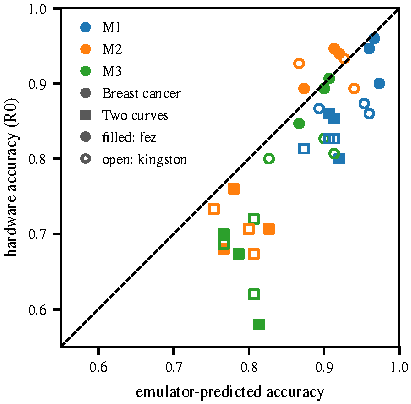
\includegraphics[width=\columnwidth]{fig3_emulator_vs_hardware.pdf}
\caption{Emulator-predicted against hardware accuracy (R0). Each point is one session, dataset
and model; colour marks the model, shape the dataset, and filled or open markers the device.
The dashed line marks equality.}
\label{fig:emu-vs-hw}
\end{figure}

\begin{figure*}[t]
\centering
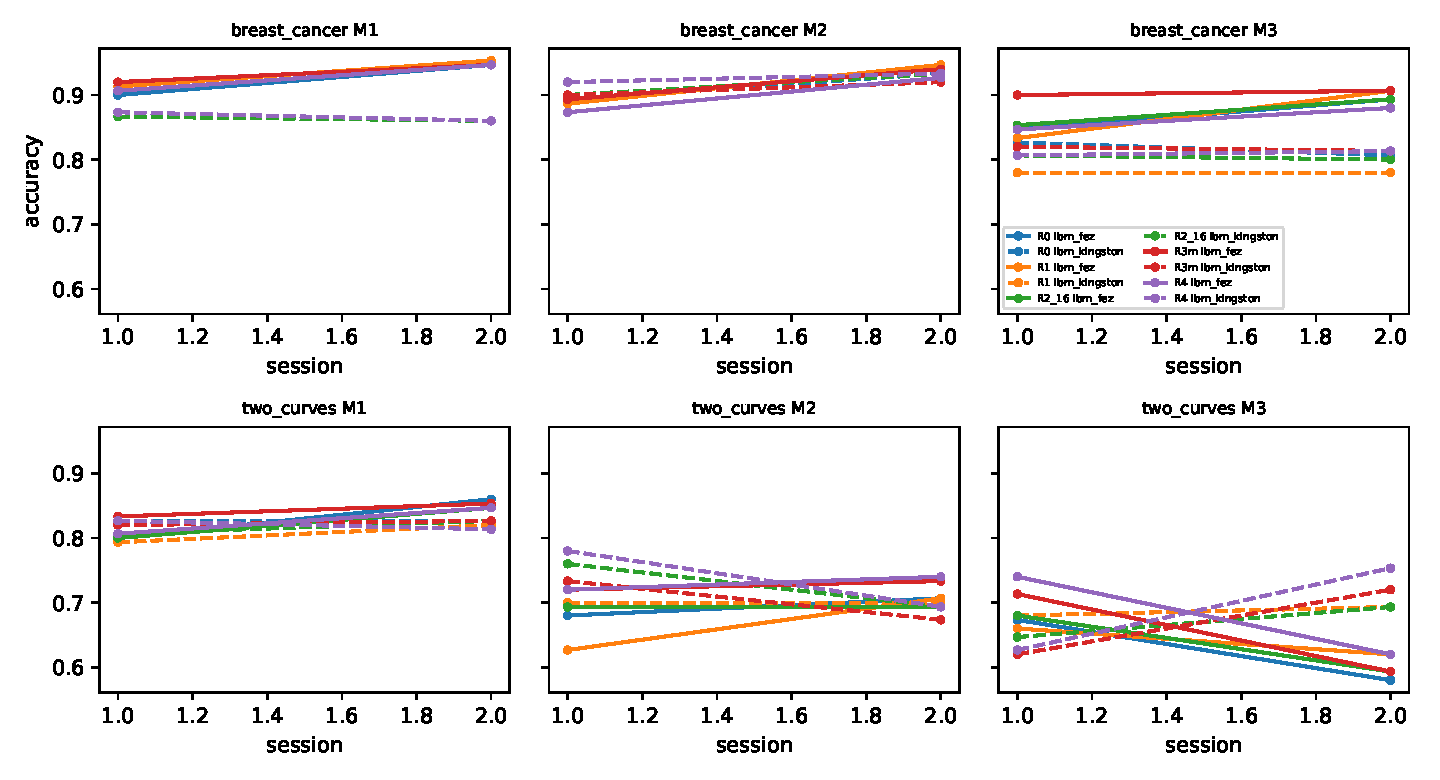
\includegraphics[width=\textwidth]{fig2_drift.pdf}
\caption{Hardware test accuracy per session for each dataset and model: R0 with 95\% bootstrap
intervals and selected repairs; solid and dashed lines are the two devices, and the dotted grey
line is the noiseless simulator.}
\label{fig:drift}
\end{figure*}

\begin{figure}[t]
\centering
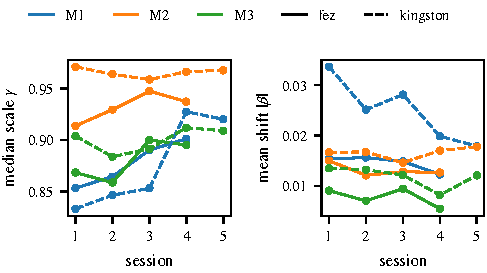
\includegraphics[width=\columnwidth]{fig4_noise_model.pdf}
\caption{Linear map from simulator to hardware features, $\phi_{\mathrm{hw}}\approx\gamma\,
\phi_{\mathrm{sim}}+\beta$, fitted per feature and session: median scale and mean absolute
shift by model and device.}
\label{fig:noise-model}
\end{figure}

\begin{figure}[t]
\centering
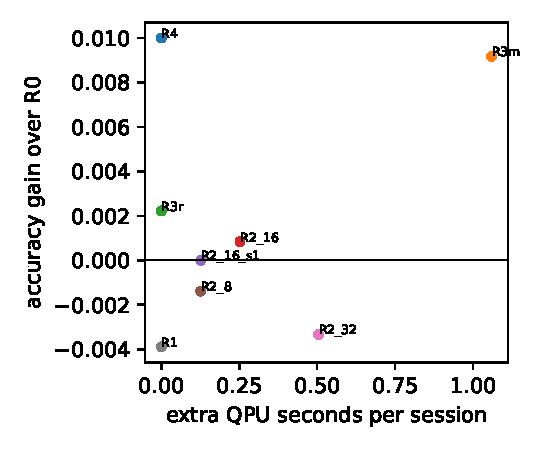
\includegraphics[width=\columnwidth]{fig5_repair_cost.pdf}
\caption{Mean accuracy gain of each repair over R0, with 95\% bootstrap intervals, against the
extra QPU seconds it needs per session. Repairs with equal cost are spread horizontally for
readability.}
\label{fig:repair-cost}
\end{figure}

\begin{figure}[t]
\centering
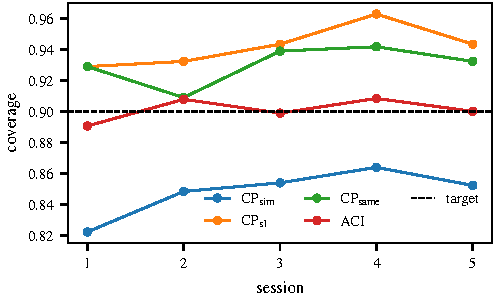
\includegraphics[width=\columnwidth]{fig6_coverage.pdf}
\caption{Conformal coverage per session, averaged over devices, datasets and models; the dashed
line is the target \val{coverage-target}.}
\label{fig:coverage}
\end{figure}

% Drafted with an AI assistant (limitations and deviations on 31 Oct, implications on 10 Nov 2026).
% Revise everything in your own words. Directional words are tagged "% claim:<id>" and are
% re-checked by `uv run qdrift paper`.
\section{Discussion}
\label{sec:discussion}

\textbf{Implications.} A calibration emulator is a useful screen but not a stand-in for
hardware. It ordered our configurations well yet overstated their accuracy by \val{h1-mean-pp}
points on average. % claim:emu-optimistic claim:emu-ranks-well
A study of calibration-aware QAOA compilation on Heron processors also found that emulators
overstated the benefit measured on hardware~\cite{qaoa2026drift}, so the bias is unlikely to be
specific to classifiers. Day-to-day drift was real but differed between devices. % claim:drift-one-device
A result from one session, such as the single day of hardware data in the adaptive conformal
study~\cite{spencer2026aqcp}, can therefore be off by several points, while repeating a run on
another day costs about \val{session-usage-mean}~s here.

Under a free budget the cheap repairs buy little. The head trained on emulated noisy features
(R4) is free and gave the largest gain and the best calibration, % claim:r4-best claim:r4-best-ece
and measured readout mitigation is the only paid repair that helped. Normalisation, part of the
QuantumNAT pipeline that raised accuracy by up to 43\% on IBM devices of
2021~\cite{wang2022quantumnat}, gave nothing here. % claim:r1-no-gain
On these processors the global scale and shift of the features is modest and stable, so the
remaining loss comes from errors that differ between inputs and qubit chains and that one global
correction cannot remove; the association of feature error with the CZ error and $T_2$ of each
chain points the same way. % claim:h4-not-readout claim:t2-negative
For uncertainty, the practical fix is to calibrate on hardware: labels from any session
restored coverage, and ACI kept it at the target with smaller sets. % claim:hwcal-over claim:aci-near

\textbf{Limitations.} On the free plan a job runs when the queue allows, not at a chosen time:
queue waits reached \val{queue-max-h}~h during the campaign (\val{queue-max-all-h}~h including
the pilots), and with one job per session the campaign holds \val{sessions-done} sessions. The
models are small (\val{n-qubits} qubits, at most \val{max-cz} CZ gates) and the study covers two
datasets with \val{n-test} test inputs per session, so the accuracy of a single session is
uncertain by several points and only effects pooled over sessions are resolved. The qubit chains
were chosen from one day's calibration and then kept fixed; this pairs the data across sessions
but means that later sessions may not use the best qubits of that day. The emulator treats each
chain on its own and contains no crosstalk, and the packing check used \val{pilot-samples} inputs
per device, enough to exclude only large crosstalk effects. Because IBM refreshes the reported
calibration often, its age at job start lay between \val{cal-age-min-h} and \val{cal-age-max-h}~h,
which makes calibration age a weak measure of drift. Finally, twirling and dynamical decoupling
were switched off by design, so the results describe raw device noise; we did not test the
repairs together with these techniques.

\textbf{Deviations from the registration.} The registration is the git tag \texttt{prereg-v1}
(\val{prereg-date}). Before the hypotheses were first evaluated on hardware data, we corrected
the analysis code so that calibration age is measured at job start instead of at the time the
snapshot was downloaded; only the age covariate of H4 is affected. The registration asked for
sessions at a similar time of day, but the queue and the author's schedule did not always allow
it: \val{sessions-day} sessions started in the daytime and \val{sessions-night} at night (India
time). \val{window-sentence} \val{sessions-sentence}

% ===================================================================== CONCLUSION
% Target: one paragraph. Restate the main findings in one sentence each, the practical advice,
% and one or two concrete next steps (more devices, longer windows, larger models, twirling on).
\section{Conclusion}
\label{sec:conclusion}
\todo{Conclusion.}


\section*{Data and code availability}
% Fill the URL and the DOI at release (Task 12).
The code, frozen models, raw counts and calibration snapshots are available at
\todo{repository URL} and archived as \todo{Zenodo DOI}. The registration is the git tag
\texttt{prereg-v1} (commit \texttt{\val{prereg-commit}}, \val{prereg-date}).

\section*{Acknowledgment}
% IBM's requested wording for work that used IBM Quantum services; keep it as is.
We acknowledge the use of IBM Quantum services for this work. The views expressed are those of
the authors, and do not reflect the official policy or position of IBM or the IBM Quantum team.
% IEEE requires AI-generated content (text, code, figures) to be disclosed here. Keep this
% sentence accurate: edit it if you rewrite the drafts, and check your course's AI policy.
The analysis software and first drafts of parts of this manuscript were prepared with the help
of an AI assistant (Kiro); the authors reviewed, revised and verified all code, text and results.

\bibliographystyle{IEEEtran}
\bibliography{generated/refs}

\end{document}
